% by Mirella M. Moro; version: January/18/2012 @ 04:16pm
% -- 01/18/2012: more discussion on SBBD + JIDM; overall revision
% -- 09/03/2010: bib file with names for proceedings and journals; cls with shrinked {received}
% -- 08/27/2010: appendix, table example, more explanation within comments, editors' data

\documentclass[jidm,a4paper]{jidm} % NOTE: JIDM is published on A4 paper
\usepackage{graphicx,url}  % for using figures and url format
\usepackage[T1]{fontenc}   % avoids warnings such as "LaTeX Font Warning: Font shape 'OMS/cmtt/m/n' undefined"

%\usepackage{cite} % NOTE: do **not** include this package because it conflicts with jidm.bst

% Standard definitions
\newtheorem{theorem}{Theorem}[section]
\newtheorem{conjecture}[theorem]{Conjecture}
\newtheorem{corollary}[theorem]{Corollary}
\newtheorem{proposition}[theorem]{Proposition}
\newtheorem{lemma}[theorem]{Lemma}
\newdef{definition}[theorem]{Definition}
\newdef{remark}[theorem]{Remark}

% New environment definition
\newenvironment{latexcode}
{\ttfamily\vspace{0.1in}\setlength{\parindent}{18pt}}
{\vspace{0.1in}}

% ALL FIELDS UNTIL BEGIN{document} ARE MANDATORY

% The following data (volume, number and page) are given by the editors prior to publishing your article
\jidmVolume{5}
\jidmNumber{1}
\jidmYear{14}
\jidmMonth{June}
\setcounter{page}{1}


% Includes headers with simplified name of the authors and article title
\markboth{A.C. Salgado and V. Braganholo}
{JIDM - Journal of Information and Data Management}
%  -> \markboth{}{}
%         takes 2 arguments
%         ex: \markboth{M. M. Moro}{Any article title}


% Title of the article
\title{LiveSync: a Tool for Real Time Video Streaming Synchronization from Independent Sources}


% List of authors
%IF THERE ARE TWO or more institutions, please use:
%\author{Name of Author1\inst{1}, Name of Author2\inst{2}, Name of Author3\inst{2}}
\author{Marcello N. de Amorim\inst{1}, Ricardo M. C. Segundo\inst{2}, Celso A. S. Santos\inst{3}}


%Affiliation and email
\institute{Universidade Federal do Espirito Santo, Brazil  \\ \email{novaes@inf.ufes.br , rmcs87@gmail.com , seibel@inf.ufes.br}
% IF THERE IS ANOTHER INSTITUTION:
%\and Name_of_the_second_institution \\
%\email{address@whatever.com}
}


% Article abstract - it should be from 100 to 300 words
\begin{abstract}
This work presents a tool that allows users to synchronize live videos from multiple sources such as YouTube or any other video streaming sources. The proposed approach to proceed the multiple camera video synchronization is based in crowdsourcing techniques, using the power of a crowd of collaborators to synchronize videos, requiring from each user the sync of only a pairs of videos. Additional sync relations are inferred from the known contributions, using transitivity properties and an appropriate structure for this inference, the Dynamic Alignment List.
\end{abstract}


% ACM Computing Classification System categories
\category{H.4.4.3}{Information Systems Applications}{Crowdsourcing} 
\category{H.3.2.7}{Human-Centered Computing}{Synchronous editors}

% Categories and Descriptors are available at the 1998 ACM Computing Classification System
% http://www.acm.org/about/class/1998/
%  -> \category{}{}{}
%         takes 3 arguments for the Computing Reviews Classification Scheme.
%         ex: \category{D.3.3}{Programming Languages}{Language Constructs and Features}
%                   [data types and structures]
%                   the last argument, in square brackets, is optional.

% Article keywords
\keywords{live video, synchronization, crowdsourcing}
%  -> \keywords{} (in alphabetical order \keywords{document processing, sequences,
%                      string searching, subsequences, substrings})


% THE ARTICLE BEGINS
\begin{document}

% This is optional:
\begin{bottomstuff}
The work is supported by CAPES and FAPES.
\end{bottomstuff}

\maketitle

\section{Introduction}
This paper extends the previous work \cite{delivesync} that won the prize of best tool in the XVI Workshop on Tools and Applications (WFA) of the XXII Brazilian Symposium on Multimedia and Web Systems (WebMedia 2016).

Multiple camera video synchronization is a research area within multimedia. Automatic video synchronization (AVS) is a form to synchronize multiple video streams. AVS can be done analysing video segments \cite{wang2014videosnapping} or audio ones \cite{su2012making}. In Schweiger et.al.\cite{schweiger2013fully} we find these and other approaches in the area. One main contribution of this paper is the description of the challenges for automatic synchronization algorithms: wide baselines, camera motion, dynamic backgrounds and Occlusions.

We propose in this work the use of crowdosurcing techniques to synchronize these videos, instead of an automatic one. Crowdsourcing\cite{howe2006rise} in our scope refers to the use of the crowd as part of a computational problem that can be solved easily by a human than by a machine. The "easily" word can mean that the human approach: is cheaper, faster or can be done more efficiently by humans.

In video synchronization, we know that humans can ful- fil all challenges presented by \cite{schweiger2013fully}. A person can identify if two videos are synchronized or not independently of occlusions, change of the background, camera motion or view point changes. The main challenge is how to use the human abilities to synchronize the videos, and permit that other persons can benefit from these contributions. So our tool uses the power of the crowd to synchronize live streaming videos and provide a form that other persons that want to watch those videos can receive both videos and synchronization info.

The remaining of this paper is presented as follows: section 2 explains our approach to synchronize videos; section 3 details our tool; section 4 presents a larger experiment to validate our tool in a more comprehensive application scenario ;and section 5 presents our final remarks.




\section{CrowdSourcing}

Crowdsourcing is often a highly structured process from an organization, drawing on the creativity and intelligence of an online community in an open, but controlled, way \cite{brabham2014crowdsourcing}. Crowdsourcing systems can be used in a variety of situations such as: Knowledge Discovery and Management; Distributed Human Intelligence Tasking Organization; Broadcast Search; Peer-Vetted Creative Production \cite{brabham2014crowdsourcing}. The CrowdSync problem can be classified as a "Distributed Human Intelligent Tasking" problem, where an organization sends task related to information analysis. This kind of system deals with an information management problem: how the crowd will use information contained in videos to generate synchronization points. A second characteristic for our problem is that we consider that the information is already available and it is unnecessary to locate it. We don't approach the problem of collecting the videos, here we consider only synchronizing them.

Synchonizing videos isn't the only way to use the crowd with videos. Several works use the crowd with other objectives on videos. Two main problems may be highlighted here: annotation and quality evaluation, but diverse works can be addressed.





\subsection{Annotation}
The paper Video Summarization via Crowdsourcing \cite{wu2011video} uses the crowd to identify the main occurrences in a video and thus generating a summary. In Efficiently Scaling up Crowdsourced Video Annotations \cite{vondrick2013efficiently} the crowd is used to annotate multiple videos. Through an interface provided by the authors, users can annotate videos using graphic tools, classifying objects in a video. Besides the annotation, which uses crowdsourcing, the paper presents a complementary approach that helps in annotating videos. Authors use annotations from the crowd as an input to an algorithm that automatically finalizes annotations from a video.

Generating Annotations for How-to Videos Using Crowdsourcing \cite{nguyen2013generating} also uses the crowd to generate annotations, however, in this case within a specific context. Authors divide the annotation task in three steps: identifying the time when important events occur; name each event; and identify frames indicating instants before and after the event, helping in the How-To.

Crowdsourcing event detection in YouTube video \cite{steiner2011crowdsourcing} focuses in generally identifying events in a YouTube video. It features processing in video playback time, to identify scene changes, and then allowing a viewer to annotate that part of the video. However, as stated by authors: "Regarded in isolation, neither of our video event analysis steps is new". Its contributions are in: (i) scalability through crowdsourcing, (ii) the nature of real time processing in a HTML5 client, and (iii) the combination of annotations for three different types of events (visual event, occurrence event and interest-based event).

A web-based video annotation system for crowdsourcing surveillance videos \cite{gadgil2014web} presents a platform for annotating surveillance videos. A supervisor selects and assigns tasks to users. The paper, despite using the term crowdsourcing	, uses the concept of outsourcing, once results from the crowd are not evaluated, neither combined to generate the result. Each individual has to watch the entire surveillance video and annotate it, falling back to the large tasks problem.

Tagging human activities in video by crowdsourcing \cite{nguyen2013tagging} uses the crowd to annotate scenes in a video, where each participant must annotate its start, end and details of its content to generate an annotation.

\subsection{Quality}
In Quantification of YouTube QoE via Crowdsourcing \cite{hossfeld2011quantification} the crowd is used when evaluating YouTube's quality of services (QoS). Each crowd individual watches videos from his home and rates his experience. An important point of the paper is the crowd filtering: in multiple tests executions, nearly 80\% of them were removed from results as they were considered to fail the evaluation. For the elimination, these techniques were applied: Golden Standard Data; Consistency Tests; Content Quests; Mixed Answers; and Application Usage Monitoring.
Video quality evaluation in the cloud \cite{keimel2012video} also presents a quality evaluation, but this time an evaluation from the actual video.

A subjective evaluation using crowdsourcing of Adaptive Media Playout utilizing audio-visual content features \cite{rainer2014subjective} presents another paper that uses the crowd to evaluate video quality. In this case, issues concerning adaptive video are evaluated. It is asked to participants to evaluate video quality, without knowing if video quality was modified or it remains the same.

\subsection{Others}
Crowdsourced Automatic Zoom and Scroll for Video Retargeting \cite{carlier2010crowdsourced} uses the crowd to identify focusing regions of a video. Viewers select a zoom area that focuses important content from the video, so when the video is watched in low resolution screens, only most important content is presented to users.

Introducing game elements in crowdsourced video captioning by non-experts, \cite{kacorri2014introducing} presents the use of game elements (gamification) in a crowdsourcing platform. In this case, the problem that needs to be solved is generating captions for multiple videos. The most significant about this paper is the use of video segments. This allows users to perform small tasks to achieve a greater goal. Gamification aspects are important as an incentive to participation, instead of monetizing tasks.


\section{Video Synchronization}
Besides studying the relation between crowds and videos segments, it is important to consider other video synchronization techniques, and that is what we now describe now in this section.

The audio analyses can be used to synchronize the video segments. Su \textit{et al.} \cite{su2012making} presents video synchronization using this approach. Fingerprints are generated for each audio, and a comparison between videos is performed. Bano \textit{et al.} \cite{bano2015discovery} also use audio as synchronization track using the chroma analysis from audio to group and synchronize audio from a same event.

There are also the approaches where video analyses is used instead of audio. Wang \textit{et al.} \cite{wang2014videosnapping}, synchronizes videos in space and time, allowing the navigation between videos by resemblance and time. The synchronization works for multiple videos and different cameras. Other important works is described by Schweiger \textit{et al.} \cite{schweiger2013fully} that a research for related papers in the area. It presents important results in automatic video synchronization, such as a technique that analyses differences between frames to find synchronization points. Furthermore, it presents the main challenges for automatic synchronization algorithms: wide baselines, camera motion, camera shaking, dynamic backgrounds and occlusions.

The use of human perception however, is not impaired by these. The human processing can overcame all these challenges and with or without the sound information. This is the principle that guided us to the proposed CrowdSync. Here we don't claim that the CrowdSync overcomes the automatic techniques, but with the crowd we find less limitations on what videos we can synchronize.

\section{Crowdsourced Video Synchronization}
\label{crowdsync}
A traditional video presentation involves a single User Device that is able to decode and present this single content (the Main Content) originated from a unique source. In a non-traditional scenario \cite{huang2013evolution}, the presentation environment is composed of multiple user devices (TV, smart phones, tablets, etc.) able to present multiple contents delivered for multiple sources. One such scenario is an user that access a web video and is able to access other correlated videos with different angles, audio and complementary information.

In this situation, the user accesses a mashup of digital contents that may have no explicit synchronization defined to orchestrate the  presentation. Mashups are applications generated by combining content, presentation or other applications functionalities from disparate sources. They aim to combine these sources to create useful new applications or services to users \cite{yu2008understanding}. This combination of services and contents however brings the following issue: how to synchronize these multiple contents for each user in its environment, since the contents are transmitted through different channels and from different sources that are not explicitly synchronized among them? To tackle this issue we use the crowd as part of our solution. They act as couplers, in other words, they are responsible for finding the synchronization points among related videos, allowing their synchronous presentation in a mashup video application.

The goal of video synchronization is to align a set of videos $\alpha$ in a common temporal line \cite{segundo2015remote}. For this purpose, consider $\alpha1$ and $\alpha2$ as two continuous videos. They are considered to be synchronized when, in a given time $T_{k}$ at the $kn^{th}$ time instant of $\alpha1$ and $T_{M}$ at the $mn^{th}$ time instant of $\alpha2$, they both correspond to the same instant in global time when they were captured, which is an instance of continuous space-time. If they are not synchronized, there is a time offset ($\Delta$) that added to the presentation of $\alpha1$ or $\alpha2$ will make them synchronous. The time offset between two videos V1 and V2 can be defined as $\Delta_{V1,V2} = b.V1-b.V2$, where "b.V" is the starting time of video V in reference to a timeline of the related videos, and $\Delta$ is the time offset between them in this timeline. Finding this $\Delta$ is the task attributed to the crowd. They are responsible for analysing the videos, finding the correlated ones and setting the $\Delta$ that makes them synchronous.

Three different Crowd Synchronization scenarios are presented next: Chunk Synchronization, Frame Synchronization and Live Synchronization. 

\subsection{Chunk Synchronization}
\label{chunk-sync}
Following the crowdsourcing approach, we can't let each crowdworker analyse all the entire videos to find all synchronization points. This would require too much effort of each crowdworker. For the current version of our CrowdSync system, we split the videos in small chunks of 5s each. This way we make each task a lot easier to each crowd member, because for each task he needs only to compare if two chunks overlaps and if they do, what is the $\Delta$ that makes them synchronous.

Figure~\ref{chunks_process} shows this synchronization method. First each video A e B is mapped in chunks of 5s. A pair of chunks is sent to a crowdworker that evaluates if there is synchronization and what is the $\Delta$ if there is any. In the example (Figure~\ref{chunks_process}), if the chunks [$C_{1}A$,$C_{1}B$] have no synchronization, we compare the next possibility [$C_{1}A$,$C_{2}B$] and so on until we find it or we compare all chunks. In the example the pair [$C_{1}A$,$C_{3}B$] contains a synchronization point. The crowdworker identifies it and discovers the time offset between them ($\Delta$). Using the value of $\Delta$ and knowing which chunks where the ones where the synchronization point was found, we can synchronize the full videos [A,B]. In the example, the final difference between the two videos [A,B] is $\Delta$ plus two times the chunk size, because $\Delta$ was found in the relation between the first chunk of A and the third of B, a difference of two chunks.

\begin{figure}[h]
	\centerline{\includegraphics[scale=0.35] {figure/chunks}}
	\caption{Chunk Synchronization Method}
	\label{chunks_process}
\end{figure}

When two chunks associated with two videos are synchronized, all the contents of these two videos will also be synchronized. This happens because as described in the introduction, we consider the videos as continuous. And if comparing all chunks from both videos, we can't find any synchronization point, those two probably have no synchronization point. We say probably, because there is a possibility that the crowd fails in its tasks. To reduce this possibility, there are measures that can be taken such as assessing the crowd for better contributions. We however do not discuss this issue in this paper, as our scope focus on the synchronization process only. Another important consideration here is that this approach can fall in the worst case when there is no synchronization point, and all chunks will be compared, and will fail. On the other hand, if there is an synchronization point, we can find it in the first comparison.

\subsection{Frame Synchronization}
\label{frame-sync}
The Frame synchronization is an enhancement proposal on top of the chunk model. Here, instead of using video chunks, each crowdworker receives the key-frames sequences from two videos that must be synchronized. This way, each worker has access to the full video at once, enhancing the possibilities of finding a synchronization point. However, as now the worker interacts with frames, if a pair of frames is identified as a possible synchronization point, its precision is reduced, making necessary a second step on the task: watch the videos based on the information provided by the two frames (each frame has a timestamp from when it which part of the video it was removed, making possible to calculate $\Delta$ such as in the chunk based one).

Figure~\ref{frames} shows the interface developed to this approach: on the top the user selects the probably aligned frames (or close ones) and plays the videos. If it is correct, he confirms the alignment, else he tries again or discard the synchronization. 

\begin{figure}[h]
	\centerline{\includegraphics[scale=0.25] {figure/frames}}
	\caption{Frame Synchronization Method}
	\label{frames}
\end{figure}

\section{Dynamic Alignment List}

To achieve video streaming synchronization was used the Remote Temporal Couplers (RTC) technique \cite{segundo2015remote} that allows to align videos from different sources. This technique collects synchronization points for pair of videos, and uses an inference algorithm to find out more relations between videos by transitivity over known relations.






The RTC technique was operationally represented as the Dynamic Alignment List (DAL), an abstract type designed to organize the relations between videos as well provide the functionalists required to store and process the relations.

The start model for the storage structure inside the DAL was a relational matrix MxM which can represent all possible relations between M videos, each position representing the $\Delta{time}$ between the initial point of a pair of videos. This matrix was reduced to a upper triangular matrix because $\forall{i,j} < M , \Delta_{i,j}$ = $- \Delta_{j,i}$ and the main diagonal was eliminated because $\Delta_{i,j}$ is always equal to zero. The $\Delta{time}$ for each couple of videos is calculated for $\Delta{i,j} = start(j) - start(i)$ where $start(X)$ returns the offset of video X from the start of the event's timeline.

These values are used to synchronize the M videos. If $\Delta{i,j} > 0$ the video $i$ starts before the video $j$, if $\Delta{i,j} < 0$ the video $i$ starts after the video $j$, and when $\Delta{i,j} = 0$ both videos start at the same time. The values are represented in milliseconds, so $\Delta{i,j} = 30$ means the video $j$ should starts 30 ms after the video $i$ starts in order to achieve their synchronization. Additionally, in cases which is impossible to determine a relation between a pair of videos, the value registered is $I$ that means impossible.

Into a collaborative scenario where users can contribute providing a $\Delta{i,j}$ for a pair of videos $(i,j)$, it is important to store all contributions, because the $\Delta{time}$ value should be calculated considering the contributions collected for that pair. In that approach the formula $\Delta{i,j} = start(j) - start(i)$  is used to calculate the $\Delta{time}$ for each contribution, and the value stored in DAL is determined processing all contributions for each pair. Moreover, the number of contributions for each pair can grow while the contribution process is active, and current $\Delta{time}$ of a pair can change while contributions are incoming.

In order to represent this model it was needed to define a structure more sophisticated then a matrix. This structure preserves the relational characteristics of a upper triangular matrix without the main diagonal, with an additional dimension related to the contributions for each relation between video pairs. However, it is implemented as a hash table, using linked lists hierarchically organized in three levels. 

\begin{itemize}

\item Level 1 - The first level is a list of video structures. Each structure has a unique identification label for a correspondent video. 

\item Level 2 - Each video structure points to a second level linked list composed by all possible relations that include its video, considering the relations in a upper triangular matrix without the main diagonal.  Thus, each node in a second level linked list corresponds to a relation between it's video represented in its root and another video.

\item Level 3 - Each relation in a level 2 list points to a third level list, in which each node represent a contribution for that relation.

\end{itemize}

Figure~\ref{dal} exemplify a data structure into a DAL with 5 videos. The videos, labeled as $A, B, C, D$  and $E$, are in the fist level linked list. Each video points to a second level list, it is possible to observe in Figure~\ref{dal}  that each second level linked list have only the relations that would exist in a single line of a upper triangular matrix without the main diagonal. Moreover, in Figure~\ref{dal} each relation, that is an element of second level list, points to a cloud that represents a third level list with all contributions for that relation.

\begin{figure}
	\centering
	\includegraphics[scale=0.8]{figures/dal}
	\caption{DAL with 5 Videos (A,B,C,D,E)}
	\label{dal}
\end{figure}

A completed DAL can provide all information needed to achieve synchronization for videos registered on it, although it is more than a data structure. DAL is an abstract datatype that provides the data structure plus a set of features that allows access, manage and process the information inside it, such as the function \textit{Infer Synchronization}. 

\textit{Infer Synchronization} can obtain additional relations by executing an inference algorithm over the current relations. This algorithm checks if is possible to find an indirect path between two videos by transitivity. For example, considering the videos $A, B$ and $C$, if the relations $AB$ and $BC$ are known, by transitivity is possible to infer the relation $AC$. This feature can reduce the number of contributions required to complete a DAL. 





\subsection{Structure}
The DAL isn't just a list as the name may suggests, it is a data structure composed of vectors and lists that are used to assist the processing of contributions of crowd workers as well as to support the generation of presentations with the synchronized videos. It was designed in order to efficiently store all relevant contributions that represent a temporal relation between a pair of videos.

Its structure is based on a Upper Triangular Matrix, although, the DAL is constructed on demand, saving space because it doesn't have any empty slot on it, turning it into a dynamic structure. In Figure~\ref{structure-dal} it is shown an instance of a DAL with five videos and its relations.

\begin{figure}[h]
	\centerline{\includegraphics[scale=0.7] {figure/DAL/dal}}
	\caption{DAL Structure}
	\label{structure-dal}
\end{figure}

The DAL starts as an array that contains in its positions the videos that are going to be related (blue squares). Each video is an object that contains a reference to the media that it represents (URI) or other DAL (creating a hierarchy), a reference to the array of relations with the other videos and an attribute with the duration ($\sigma$) of the video.

These relations are cells into an array. Each position of this array is a different relation that represents the time offset between those two videos. Each position of the array stores the IDs for the pairs of videos that are being related, an attribute that contains the current $\Delta$ (time offset), an attribute that contains the degree of confidence in that relation and a list of contributions on that relation (each contribution on which is the $\Delta$ value). The degree of confidence is how precise the current $\Delta$ is believed to be true. Note that we don't need to store all direct relations (e.g. $\Delta_{A,H}$ and $\Delta_{H,A}$), we can store one direct relation and its complementary can be easily calculated ($\Delta_{A,H} = -\Delta_{H,A}$).

A contribution (in the blue cloud) in turn has the $\Delta$ proposed by each user for that relation and a reference for that user (the user profile may be used to rise the degree of confidence of a relation).

\subsection{Time Offset Management}
The first feature (and original purpose) of the DAL is the Time Offset Management. It is responsible for dealing with all aspects of the time offset relation among videos. These aspects are:

	\textbf{$\Delta$ Storage and Retrieval:} a characteristic of the DAL is to allow the addition, update and retrieval of any Time Offset for any pair of videos. This gave us the starting point of using a Matrix like structure that permits fast access to any cell of the matrix  from a pair of coordinates. This way knowing the two videos which we desire to know or to update the $\Delta$, we can quickly obtain this information. However we don't use a pure matrix for two main reasons: information redundancy, we don't need to store the AB and BA relations, as one is the opposite of the other ($\Delta_{i,j} = -\Delta_{j,i}$, eq.~\ref{eq-oposite}); and a matrix doesn't allow the storage of multiple contributions in the same cell (requisite for the crowdsourcing);
\begin{eqnarray}
	\label{eq-oposite}
	\Delta_{i,j} = b.i - b.j	\nonumber \\
	\Delta_{j,i} = b.j - b.i	\nonumber \\
	-\Delta_{j,i} = b.i + b.j	\nonumber \\
	\Delta_{i,j} = -\Delta_{j,i}
\end{eqnarray}

	\textbf{$\Delta$ Inference:} known relations in the DAL allows developing inference methods that use transitivity through pairs of aligned videos to calculate relations between videos,in which the offset is still unknown. If we know the relation AB and AC from the structure we can infer BC.	
\begin{eqnarray}
	\label{dina-i}
	\Delta_{B,C} = b.B - b.C	\nonumber \\
	\Delta_{B,A} = b.B - b.A \rightarrow b.B = \Delta_{B,A} + b.A	\nonumber \\
	\Delta_{A,C} = b.A - b.C \rightarrow b.A = \Delta_{A,C} + b.C	\nonumber \\
	\Delta_{B,C}= \Delta_{B,A} + b.A - (b.A-\Delta_{A,C}) \rightarrow \nonumber \\ \Delta_{B,C} = \Delta_{B,A} + \Delta_{A,C}	
\end{eqnarray}

	\textbf{Presentation Generation:} With the known and inferred time offsets, it is possible to create a presentation of the event that correlates all videos with temporal relations. This presentation can be the maximal one, where the event is presented using the first video until the end of the last one, also when videos with overlapping exists, the option to change camera is made available to users.

\subsection{Contribution Management}
The Contribution Management is a requisite in order to adequate the DAL for a crowdsourced scenario. It is necessary to receive, distribute and process the crowd contributions in order to find the correct Time Offsets. The aspects involved in the Contribution Management are:

	\textbf{Convergence:} one of the principles of crowdsourcing is collecting the contribution of multiple members and based on these contributions finding the solution to a problem. In our case, the crowd watches the videos fragments and find synchronization points. The convergence is responsible for getting all theses contribution, and merging them in actual results.
	
	The Convergence Level detects the tendency of the Crowd about the Relation of a pair of videos. This tendency is an indicative of the agreement on a Delta between the videos. According to the scenario, a Convergence Threshold that is used to determine if a Relation is converged, is defined. Each Relation have an attribute that stores its current convergence level. If this level reaches a Convergence Threshold the method returns True, otherwise it returns False.

	Initially all Relations are created with Convergence Level 0, and consecutive similar contributions increase this value. If a tendency change in the contributions is detected, the Convergence Level is reset.
	
	\textbf{Video Selection:} the convergence deals with the problem of receiving and processing the crowd contributions. However, we must correctly choose the videos to be evaluated by the crowd that results in a contribution. The selection of these videos is part of the contribution management. 
	
	This method intent is to select which pair of videos should have priority to receive contributions. It consists of a sequence of two other methods: (i) Choose the next Video; (ii) Choose the next Relation. When this method returns NULL, it means that the DAL has been converged.
	
In order to increase possible inferences over the contributions, the method try to spread contributions over the timeline, proceeding a random selection among the Videos that were not converged nor marked as a Impossible relation. Once a Video is chosen the method select from its Relations array the Relation closer to converge.

\subsection{Convergence Criteria}
\input{convergence}

\subsection{Inference Algorithm}
\input{inference}

\section{LiveSync}
Live synchronization includes the scenario where a viewer has access to an event that is live streamed by more than one Content Provider. These content providers are independent, so their videos do not have initial resources that allow their automatic synchronization to viewers, requiring a video analysis to generate synchronization points (Couplers). This synchronization fits as a problem that can be solved by using the power of the crowd. This occurs because videos are generated independently, without synchronization points and without previous description of what is about to be shown in screen, neither how can it be correlated to other videos. This way, human perception is used in real time to generate unknown synchronization points. 

As example for this scenario, we can take a public manifestation. In the event, multiple people can take their cell phones and start streaming the event. In their house, other people can watch the videos. However, the multiple videos from different sources will be asynchronous. We need a way to synchronize these UGV. We use the crowd to achieve it. To this objective we group all videos in a MashUp application that connects to a Coupler Server that contains all synchronization data. Both synchronizing and playing the videos are made using this mashup, that can receive videos from multiple sources.






%%%%%%%%%%%%%%%%%%% ACM %%%%%%%%%%%%%%

Live synchronization includes the scenario where a viewer has access to an event that is live streamed by more than one Content Provider. These content providers are independent, so their videos do not have initial resources that allow their automatic synchronization to viewers, requiring a video analysis to generate synchronization points (Couplers).

As example for this scenario, we can take a public manifestation. In the event, multiple people can take their cell phones and start streaming the event. In their house, other people can watch the videos. However, the multiple videos from different sources will be asynchronous. We need a way to synchronize these UGVs. We use the crowd to achieve it. To this objective we group all videos in a mashup application that connects to a Coupler Server that contains all synchronization data. Both synchronizing and playing the videos are made using this mashup, that can receive videos from multiple sources.

In a live presentation, it is assumed that content must be consumed right after its generation. It is of extreme importance that the synchronization method can be performed in playback time, to allow the integration of live content. However, not all viewers are required to be part of the crowd to achieve synchronization. If a synchronization made by a single member of the crowd is accepted as accurate, it can be transferred to the remaining viewers, this way each one will have his content locally synchronized.

One way of live synchronization can work is as follows: a person selects and synchronizes two videos with the help of a manipulation tool. This becomes a candidate synchronization point. Several people can do the same, and the results can be based on multiple synchronizations. Having these synchronization points defined, synchronization information can be sent to other viewers interested in watching those videos. As simple example, take two independent sources that are transmitting an event. A mashup system allows the user to watch both videos at the same time is his device. However the videos are asynchronous and the user notices that. He then access the option to synchronize the videos. After he achieve a synchronous result, implicitly his contribution is sent to a server that will feed other users that choose to watch the same videos with the synchronization specification. If the user thinks the content is not synchronised yet, he can synchronize it himself and send another contribution. This tool was implemented and is presented on section~\ref{livesync}.







\subsection{Method}
\input{method}

\subsection{LiveSync Tool}
\label{livesync}
The main functionalities provided by our tool are:

\textbf{Synchronized Live Video Player:} The tool permits users to watch multiple videos synchronized. He selects from a list of sources the videos he wishes to watch and them they are synchronized using information provided by other users. If a pair of videos does not have any information about their synchronization, users are invited to contribute and synchronize the videos.

\textbf{Synchronization Infering:} In some cases that there is no direct information about the synchronization of two videos, the tool is able to infer the synchronization about them, based on the contributions of other videos. We use the transitive attribute of video synchronizations, where if we know AB and BC synchronization info (couplers), we can infer AC. To infer this value we travel trough the DAL, finding the unknown relations (for example, CE), and try to find a path of known relations where we can infer CE. Taking the DAL in Figure 1, we can infer CE if we know: AC and AE. This a two steps route, but we try all possible routes when inferring, in a way that we fill as much relations as possible.

\textbf{Video Aggregation:} Although the focus of the LiveSync tool is on synchronization, we allow users to add new stream sources to the application. He only needs to set the video source, and the video will be added to the DAL and list of videos. However, we don't do any filtering about the added video, this means that the user can add any video to the application, even ones that contains none relation with the other videos. In future versions we plan to add options where other users can mark the video as not related, and then remove them.

\textbf{Multiple Video Platform Support:} One keypoint of our tool is the use of other platforms as video sources. The videos that we play to users and that are synchronized, are not provided by us, but by other live video stream platforms. To be compatible with our tool, two requisites are required:

\begin{enumerate}
	\item Remote Player: we need that the platform allows embeddable players on third pages, allowing us to control the player with its basic functionalities such as: play, pause and stop;
	\item Uptime Support: a second and fundamental requisite is an API that allows us to retrieve the video Uptime. Video uptime is the time since the beginning of the video that is presented on the video player. This is fundamental to create and replicate the couplers generated in synchronization process.
\end{enumerate}

\textbf{Serverless Architecture:} Serverless architectures refer to applications that significantly depend on third-party services and putting much of the application behavior and logic on the front end. Such architectures remove the need for the traditional server system sitting behind an application.

\textbf{Multiplatform:} LiveSync is a Web Based application designed and developed in compatibility with HTML5 standard to its front-end (Mashup Player) component. It allows our application to run on multiple browsers, operational systems and devices.

\textbf{Active X Passive Contributions:} Two branches of the LiveSync are currently on our repositories. They differ only in one aspect: who defines what videos are to be synchronized: the crowd or the application? The active version allow users to navigate freely through the videos, synchronizing them when they wish to. The focus of this branch is to allow users to contribute if they want to. On the other hand, in the Passive branch the server gives the crowd exactly what video they will synchronize. The focus here is to rapidly synchronize all videos, so the focus isn’t to make users watch the videos, but force them to synchronize all the base for other porpoises. The active branch is the focus here, but can easily converted to the passive one.


\subsubsection{Main Functionalities}
\input{main_funcionalities}

\subsubsection{Architecture}


The LiveSync tool has three main components (Figure~\ref{live_arq}): the Content Providers (Video Sources), the Coupler and the Mashup Player.

\begin{figure}[h]
	\centerline{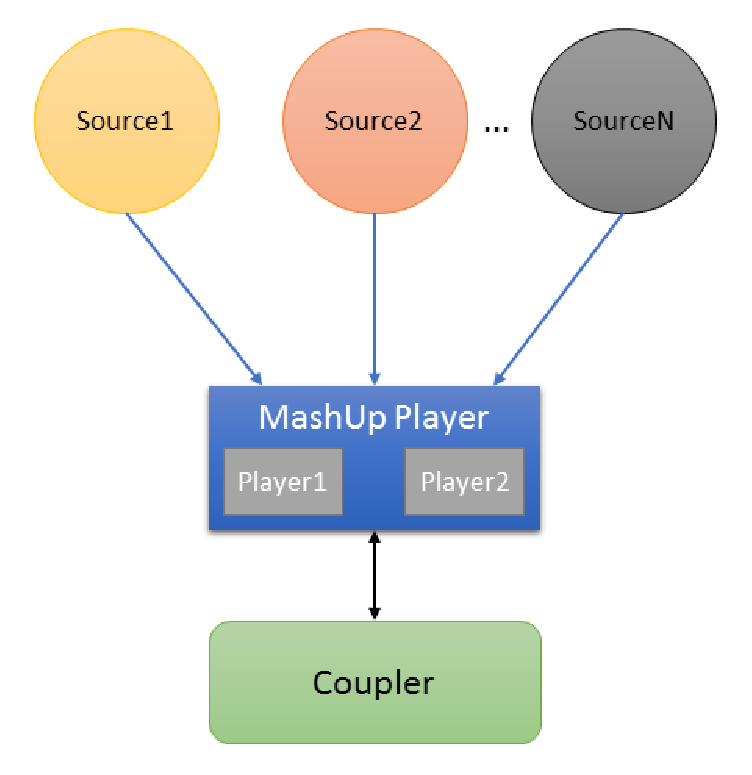
\includegraphics[scale=0.6] {figure/arqchitecture}}
	\caption{LiveSync Model}
	\label{live_arq}
\end{figure}




\subsubsection{Content Providers}
Content Providers are third-parties videos streamers platforms. There are multiple Live Video Stream applications in the market, such as YouTube Live, LiveStream, TwitCast, Twitch and Ustream. One of our objective was to allow the use of different platforms as video sources, so we maximize the number of videos for an event and allow the use of already in market platforms. 

A Content Provider needs two requisites to be compatible with LiveSync: a Remote Player and Uptime Support. As each stream platform uses their own protocols, we opt to use their embeddable players into a MashUp application. These players must allow us to play, pause and stop the video stream. The second requisite, Uptime Support, is necessary to find the couplers among the videos. Uptime is the time passed since the beginning of the live stream until the video part being presented in the player at the moment of the call.

At this time, LiveSync supports two video stream platforms: the YouTube Live (https://goo.gl/DEM9eW) and WebSocket Stream (http://goo.gl/GYnGpg). YouTube live allows live stream from both desktop and mobile devices, making possible users to stream any event they wish with low effort: they only need to install the software and to have a YouTbe account. WebSocket Stream is an open source project that allows developers to implement live stream services with websockets and canvas and WebGl technologies. It works in any browser and was used for our first tests where we needed full control of the stream, something that YouTube Live doesn't support.

To add an video source form a Content Provider, it necessary only the video ID from YouTube Live or the video stream URI from the WebSocket Stream. These are added as assets to the LiveSync and can be accessed or synchronized.


%%%%%%%%%%%%%%%%% ACM %%%%%%%%%%%%%%

%\textbf{\textit{Content Providers}}

%Content Providers are third-parties videos streamers platforms. There are multiple Live Video Stream applications in the market, such as YouTube Live, LiveStream, TwitCast, Twitch and Ustream. One of our objective was to allow the use of different platforms as video sources, so we maximize the number of videos for an event and allow the use of already in market platforms. A Content Provider needs two requisites to be compatible with LiveSync: a Remote Player and Uptime Support. As each stream platform uses their own protocols, we opt to use their embeddable players into a MashUp application. These players must allow us to play, pause and stop the video stream. The second requisite, Uptime Support, is necessary to find the couplers among the videos. Uptime is the time passed since the beginning of the live stream until the video part being presented in the player at the moment of the call.

\subsubsection{Coupler}
The Coupler is responsible for storage, distribution and calculation of synchronization points among video streams from the Content Providers.

A coupler is composed of a DAL instance and Log files. This goes in direction of the Serverless Architecture. We wanted an architecture that needed low resources (another justification for using third party stream services) and easy deployment. All that is necessary do execute the coupler is a NODE.JS (https://nodejs.org/en/) server instance. This is possible because the Coupler is fully developed in JavaScript and compatible with the HTML5 standards. To deploy the Coupler, we use a Backend as a Service or "BaaS" platform, more specifically we use the Heroku (www.heroku.com) one, that permits free use of NODE.JS instances.

It stores synchronization information only during the duration of the event, so its stance is finished with the end of the videos and all data is lost. In the current scope, the sync info is only necessary during the event, after it, there is no need to store the information. For reasons of testing and using the filmed videos from YouTube we create log files that contains all contributions made by the crowd. If it is important to maintain all contributions and data for post analyses and further use, unstable version of the LiveSync is being configured to use a fully transactional database. We use a fully transactional database because we want to maintain track of all contributions made by the crowd, an important aspect in crowdsourcing and that is also supported by the DAL.

Other aspect of the Coupler is that it is responsible for the distribution of synchronization couplers. When a user chooses two videos, a message is sent from the MashUp to the coupler, containing the required relation. The coupler then answer with the required information. If the relations is unknown, it answer soliciting the user to synchronize and contribute with those two videos.

The last function of the Coupler, is to calculate the synchronization points among Videos. Each relation ($\Delta_{A,B}$) may contain several contributions, then it is necessary to calculate a value to that relation based on the contributions. In the current version we calculate a Geometric Mean of the contributions to find an ideal value. This however may not be the best value, because the more accurate the sync is, the better the results are, so older contributions must have a lighter weight, something that does not happen in current version. The other calculation made by the coupler, is to infer unknown relations based on the afore mentioned transitive relation.

The communication  between Coupler and MashUp is made through Websocket communication. The MashUp creates a WebSocket channel with the Coupler, and requests the sync information or sends contributions from the crowd. A simple protocol is used in JSON messages: {act:value, data:object}. The act field contains the action to be made and the data contains an object to complement the action. As example we have an act to send a new contribution ("contribution") that is complemented with a new relation that contains the assets involved, the value and an id to that contribution.


%%%%%%%%%%%%%%%%% ACM %%%%%%%%%%%%%%%

\textbf{\textit{Coupler}}

The Coupler is responsible for storage, distribution and calculation of synchronization points among video streams from the Content Providers.

A coupler is composed of a DAL instance and Log files. This goes in direction of the Serverless Architecture. We wanted an architecture that needed low resources (another justification for using third party stream services) and easy deployment. All that is necessary do execute the coupler is a NODE.JS (https://nodejs.org/en/) server instance. This is possible because the Coupler is fully developed in JavaScript and compatible with the HTML5 standards. To deploy the Coupler, we use a Backend as a Service or ”BaaS” platform, more specifically we use the Heroku (www.heroku.com) one, that permits free use of NODE.JS instances.

It stores synchronization information only during the duration of the event, so its stance is finished with the end of the videos and all data is lost. In the current scope, the sync info is only necessary during the event, after it, there is no need to store the information. For reasons of testing and using the filmed videos from YouTube we create log files that contains all contributions made by the crowd. If it is important to maintain all contributions and data for post analyses and further use, unstable version of the LiveSync is being configured to use a fully transactional database. We use a fully transactional database because we want to maintain track of all contributions made by the crowd, an important aspect in crowdsourcing and that is also supported by the DAL.

\subsubsection{MashUp Player}
Mashups are applications generated by combining content, presentation or other applications functionalities from disparate sources. They aim to combine these sources to create useful new applications or services (the offer and consumption of data between two devices) to users \cite{yu2008understanding}. In LiveSync we combine videos coming from different sources and platforms with the synchronization information from the coupler to reproduce a synchronous presentation of these videos.

The MashUp Player (Figure 3) is responsible for both presenting video synchronously and collecting the synchronization. Figure~\ref{screen1} represents the interface of the MashUp.

\begin{figure}
	\centerline{\includegraphics[scale=0.17] {figure/screen}}
	\caption{Modelo simplificado do live-sync}
	\label{screen1}
\end{figure}

On the top we have all information necessary to the user. He can aggregate new videos using the ADD NEW VIDEO options, SYNCHRONIZE the videos if he thinks the videos are not synchronized or he can just select the videos he want to watch. When just playing two selected videos from the videos list, each video player creates an instance for the player that is compatible with that source (YouTube or WebSocket). It is invisible to the user where the video is coming from.

When the user adds a video, an input text is shown to him, and he can add the video URI (WebSocket) or video ID (YouTube). The page reloads and the new video is listed in the video list for everyone that connects to the application. When the video is added by the user, an message is sent to the Coupler, containing the action to add a new asset to the DAL, and the specification of it, such as label and URI.

The last functionality of the MashUp is to synchronize the videos. When the user clicks on SYNCHRONIZE, a new mode of the application is revelled showing the synchronization tools. We use a Play 'n Pause approach to synchronize the videos. After the user thinks the videos are synchronized, clicking the DONE button, his contribution is sent to the Coupler and stored in the DAL for further processing of the relation.

\textbf{\textit{Play 'n Pause:}} If two videos with a certain degree of similarity, are presented to an individual from the crowd, he can possibly notice that one video is ahead of the other. This way, he can pause the video that is ahead on time while the other remains playing, until reaching a point of synchronization. Then, the user can resume playback of the first video. This process can be repeated until an individual feels like both videos are being presented synchronously. On \url{https://goo.gl/HTzecL}, readers can see the play and pause technique being used to synchronize two live streams from from Two YouTube servers.




%%%%%%%%%%%%%%%%%%%% ACM %%%%%%%%%%%%%%%%

\textbf{\textit{MashUp Player}}

Mashups are applications generated by combining content, presentation or other applications functionalities from disparate sources. They aim to combine these sources to create useful new applications or services (the offer and consumption of data between two devices) to users. In LiveSync we combine videos coming from different sources and platforms with the synchronization information from the coupler to reproduce a synchronous presentation of these videos.

The MashUp Player (Figure~\ref{live_tvs}) is responsible for both presenting video synchronously and collecting the synchronization. Figure~\ref{live_tvs} represents the interface of the MashUp during a test: two cameras live streaming (content providers) a simulated television event to our mashup application.

\begin{figure}[h]
	\centerline{\includegraphics[scale=0.2] {figure/screen}}
	\caption{Live Streams from Olympic Games Synchronized through two different cameras}
	\label{live_tvs}
\end{figure}

On the top we have all information necessary to the user. He can aggregate new videos using the ADD NEW VIDEO options, SYNCHRONIZE the videos if he thinks the videos are not synchronized or he can just select the videos he want to watch. When just playing two selected videos from the videos list, each video player creates an instance for the player that is compatible with that source (YouTube or WebSocket). It is invisible to the user where the video is coming from.

When the user adds a video, an input text is shown to him, and he can add the video URI (WebSocket) or video ID YouTube). The page reloads and the new video is listed in the video list for everyone that connects to the application. When the video is added by the user, an message is sent to the Coupler, containing the action to add a new asset to the DAL, and the specification of it, such as label and URI.

The last functionality of the MashUp is to synchronize the videos. When the user clicks on SYNCHRONIZE, a new mode of the application is revelled showing the synchronization tools. We use a Play ’n Pause approach to synchronize the videos. After the user thinks the videos are synchronized, clicking the DONE button, his contribution is sent to the Coupler and stored in the DAL for further processing of the relation.

\section{Experiments}
Aiming to verify the CrowdSync method and the data structure generated to implement the method, two different experiments were executed:

\begin{description}
	\item[LiveSync Tool:] the LiveSync Tool implements all requisites for live synchronizing live UGV streams. Its objective is to allow the creation of mash applications of related video streams with client based solutions.
	\item[Crowd Simulated DAL:] the second experiment uses a simulated crowd to verify the DAL. The objective here is to verify if the DAL correctly stores, infers, converges and selects videos and relations. We simulate the crowd so we can make a controlled analysis in a set of videos with different crowd profiles.
	\item[UGV Dataset Synchronization:] in the third experiment, real users (crowd workers) synchronize a user generated video dataset using a developed platform with all characteristics described in this paper. Since the simulated experiment allows only to verify the correct functioning of the algorithms and structure, the focus here is to verify if humans using their perception can find the synchronization points in all related videos.
\end{description}






\subsection{Crowd Simulated DAL}

In order to validate the DAL it was designed a way to simulate a crowd, that allows us to run multiple experiments with large datasets in a viable time and without the possible biasing issues that can occur when using a human crowd. The solution found was to create the Crowd Simulator, a parameterized system that can simulate crowds with different levels of reliability, providing many contributions in short time.

To determine how the Crowd Simulator should work, we had to understand the behavior of the crowd. Yu et al.\cite{yu2012challenges} classify the crowd in four categories: Hon workers: honest worker agents who return high quality HIT (human intelligence task) results randomly 90\% of the time; MH workers: moderately honest worker agents who return high quality HIT results randomly 70\% of the time; MM workers: moderately malicious worker agents who return high quality HIT results randomly 30\% of the time; Mal workers: malicious worker agents who return high quality HIT results randomly 10\% of the time. In our scenario we consider a high quality HIT as a positive synchronization point identification or correct negation.

Per these definitions, the Crowd Simulator is settled with the percentage of honest workers in the simulated crowd, and we name this parameter as Crowd Trustworthy Degree. Each time the simulator is called, it determines the current worker reliability as so the chance of his contribution represents a high quality answer. As the objective of this experiment is validating de DAL, each high quality result is extracted from a Gold Standard Table that contains all relations between videos in dataset.

For this experiment we used the Climbing video dataset \cite{hal-01162603} that contains 89 videos captured from several different devices and users in order to register a climbing activity by distinct points of view. This climbing event has 4327.3 seconds long, and the videos starts in different offsets with durations varying between 18.96 and 1259.06 seconds. We made tests for 11 Crowd Trustworthy Degrees (from 100\% to 0\%) running 30 full simulations for each degree. Table 1 presents, for each Crowd Trustworthy Degree, the median of how many contributions were needed to converge the DAL (find all time offsets) after 30 roll of the simulation, the number of relations found, and the error rate.

As the dataset contains 89 videos, the goal was to find all 3916 relations for all pairs of videos in it. To reduce the false convergences, we used the convergence level three to determine that a value is assumed correct, this means that at least three sequential agreements are necessary to converge a value.

We also created a Gold Standard DAL built with 100\% of correct answers from de Gold Standard Table (available with the dataset), allowing us to compare the DAL generated in each run with the Gold Standard DAL for accuracy and efficiency of the simulated crowd.  Table~\ref{xp1} shows the results of the simulation. Each line corresponds to a test with different Trustworthy Degrees (reliability).  Besides the reliability, each line presents the number of necessary contributions to converge, the total amount of possible relations (not all relations will present values, as there may be GAPs among videos) found among pairs of videos and the error degree.


\begin{table}
\begin{center}
\caption{Median for all 89 Videos, after 30 rolls of simulations for each Trustworthy degree} \label{xp1}
\begin{tabular}{|c|c|c|c|}
  \hline
  Reliability & Contributions & Relations & Error
  \\
  \hline
  100\% & 11161 & 1115 & 9\% \\
  90\%  & 12101 & 1095 & 10\% \\
  80\%  & 13199 & 1095 & 10\% \\
  70\%  & 14475 & 1082 & 12\% \\
  60\%  & 16077 & 1069 & 12\% \\
  50\%  & 18015 & 1056 & 13\% \\
  40\%  & 20500 & 1052 & 14\%\\
  30\%  & 23904 & 1040 & 15\% \\
  20\%  & 28404 & 1038 & 15\% \\
  10\%  & 35121 & 1002 & 18\% \\
  0\%   & 46356 & 975  & 21\% \\
  \hline
\end{tabular}
\end{center}
\end{table}

Analyzing the result, we can see that the number of relations found don’t decrease significantly when the reliability of the crowd declines, also the percentage of the wrong relations found don’t raises dramatically. The major change among the different reliability degrees is on the number of necessary contributions to converge a DAL.

As can be seen in Figure~\ref{results-line}, between Crowd Trustworthy Degree 100\% and 50\% the results decrease linearly, below 50\% the result quality decline faster.

\begin{figure}[h]
	\centerline{\includegraphics[scale=0.8] {figure/results-line}}
	\caption{evolution of results by each between Crowd Trustworthy Degree}
	\label{results-line}
\end{figure}


\subsection{UGV Dataset Synchronization} 
Instead of discarding the human factor, this experiment aims at testing if the human factor is able to find and synchronize an User Generated Video dataset. The Climbing video dataset \cite{hal-01162603} presents multiple videos filmed by a group during a climbing activity. The automatic technique presented with the dataset presents some limitations making this dataset ideal to test the crowd approach, so we selected part of the dataset (9 videos) to our experiment. The automatic method could identify 23\% of all pairs of videos that temporally overlap, the pairwise alignment score (PAS).

To execute our experiment, we developed the technique described in section~\ref{chunk-sync}, where the crowd member analyse video chunks (5s) pair by pair, identifying if there is relation and the precision of the relation if one exists. This was the chosen solution because requires less effort from the crowdworkers, and more detailed tests are necessary to evaluate the Frame Synchronization one, as a more complex task may compromise the worker activity.

From the known ground-truth we analysed the values resulted from the crowd to evaluate the alignment within a tolerance of 0.5s \cite{hal-01162603}. The comparison with the ground truth resulted in 88\% (PAS) of correct relations among the videos. The nine videos generated 278 chunks of video (a total of 1390 seconds to be synchronized) demanding a total of 1051 contributions. Most of these (99\%) contributions were negative ones, in other words, the crowd worker could not identify synchronization  point. This indicates that most of the crowd effort is being done in discarding synchronization point, and not really finding them.

Figure~\ref{interface} shows an instant where overlapping occurs in videos recorded using 6 different cameras are synchronously presented after the crowd contributions. The other three ones are not shown because in this instant no overlapping was indicated by the crowd. It is possible to notice how heterogeneous are the camera shots. 

\begin{figure}[h]
	\centerline{\includegraphics[scale=0.2] {figure/matrix}}
	\caption{Synchronized Video Matrix}
	\label{interface}
\end{figure}

\section{Final Remarks}
The LiveSync tool allows users to watch live video streams from multiple sources synchronized. If the videos are not synchronized, user can contribute and synchronize them- selves the videos and help building the synchronization, in a crowdsourced approach, believing that using human per- ception is better than using automatic approaches in this specific case.

Our tool however presents some limitations that shall in the futures be suppressed, such as the number of events that we can follow. Now, each instance of Coupler and MashUps can handle only one event, in other words, we can’t cover two independent live events at the same time with one instance, for that porpoise we need more than on instance of each service. Also, new stream services must be added to increase our compatibilities.

Github \url{https://github.com/rmcs87/liveSync} contains all code for LiveSync.


%%%%%%%%%%%%%%%%% ACM %%%%%%%%%%%%%%%

Crowds can be used in the most diverse situations: from designing a product to digitizing a word, going through most diverse scenarios, as discovering the structure of a protein. Exploring this variety of uses of the crowd this paper presented the possibility of using crowds in the video synchronization process. Using the crowd allows to address challenges that automatic processing techniques struggle to solve, like: moving cameras, constantly changing backgrounds, disappearing objects and others. A human can handle this problems without affecting his perception about a video

Nevertheless, using crowdsourcing techniques also introduces new problems to the process: which pair of videos will be sent to each user? Where are the contributions stored? How can the contributions be validated? How to know that all videos are synchronized? What are the time offsets among the videos? Do I need to compare all videos? As solution to these problems the DAL was described. An structure that can manage temporal relations and crowd contributions.

The first experiment showed the simpler where the crowd can be used: the live one. It is said simpler because the crowd has a smaller search area to find the videos alignment point. With the LiveSync this scenario can be solved and multiple mashups applications developed. The Second experiment showed us that the more reliable the crowd is, the less contributions we need and that 100\% to 60\% may generate similar results. Also we don't need the crowd to find all values: most of the relations we can infer from others. The third experiment showed us that it is possible to use the power of the crowd to synchronize video datasets, in the a hard dataset that presented challenge even to automatic solutions. From the second experiment we also learned that most contributions are to find that two chunks don't have a synchronization point. This is important and is the key point to the next steps in the development of our research, as we are developing new interfaces that helps the crowd members in identifying the synchronization points in entire videos at once, not only chunks. This will lead us in reducing the number of required contributions and achieve more accurate results.

All code involved in our research is opensource and is available in [Removed for Blind Review].

% INCLUDE BIBLIOGRAPHY WHICH MUST FOLLOW jidm.bst TEMPLATE
\bibliographystyle{jidm}
\bibliography{jidmb}
% For information on how to write bibliography entries, 
% see file jidmb.bib

\end{document}
